\documentclass[]{article}

%Used to improve the headers
\usepackage{fancyhdr}

%Used to include images into the document
\usepackage{graphicx}

%Used to make some pages landscape
\usepackage{lscape}

%Used to wrap figures in text
\usepackage{wrapfig}

%Translate LaTeX terms to dutch
\usepackage[dutch]{babel}

%Used to display url's
\usepackage{hyperref}

\usepackage{longtable}

%Used to display "normal" paragraph's without indentation and with blank line
\usepackage[parfill]{parskip}

%Use \insertdate to insert current formatted date
\makeatletter
\let\insertdate\@date
\makeatother

%add version command, use \version to insert current version
\newcommand{\version}{1.05}

% Alter some LaTeX defaults for better treatment of figures:
% See p.105 of "TeX Unbound" for suggested values.
% See pp. 199-200 of Lamport's "LaTeX" book for details.
%   General parameters, for ALL pages:
\renewcommand{\topfraction}{0.9}    % max fraction of floats at top
\renewcommand{\bottomfraction}{0.8} % max fraction of floats at bottom
%   Parameters for TEXT pages (not float pages):
\setcounter{topnumber}{2}
\setcounter{bottomnumber}{2}
\setcounter{totalnumber}{4}     % 2 may work better
\setcounter{dbltopnumber}{2}    % for 2-column pages
\renewcommand{\dbltopfraction}{0.9} % fit big float above 2-col. text
\renewcommand{\textfraction}{0.07}  % allow minimal text w. figs
%   Parameters for FLOAT pages (not text pages):
\renewcommand{\floatpagefraction}{0.7}  % require fuller float pages
% N.B.: floatpagefraction MUST be less than topfraction !!
\renewcommand{\dblfloatpagefraction}{0.7}   % require fuller float pages

\pagestyle{fancy}

\fancyhead{}
\fancyfoot{}

\fancyhead[L]{Melroy van den Berg \& Vincent Kriek}
\fancyhead[R]{
\includegraphics[height=30pt,keepaspectratio]{tassbw.pdf}}

\fancyfoot[L]{Afstudeerverslag}
\fancyfoot[C]{\thepage}
\fancyfoot[R]{v\version}

% Add line above footer
\renewcommand{\footrulewidth}{0.4pt}% default is 0pt

\begin{document}

\title{Afstudeerverslag}
\author{Vincent Kriek \and Melroy van den Berg}

\maketitle

\vspace*{\fill}

\begin{tabular}{|| l | l || l | l ||}\hline
   Document ID: & AFVSL-MV-21          &Project naam:     &DomoTop             \\\hline
   Datum:       &4 april 2012          &School begeleider:&Peter Kailuhu       \\\hline
   Versie:      &\version              &People Manager:   &Gerben Blom         \\\hline
   Status:      &concept               &Documentnaam:     &Afstudeerverslag.pdf\\\hline
   Auteur:      &Melroy van den Berg \&&Reviewer:         &Gerben Blom         \\
                &Vincent Kriek         &                  &                    \\\hline
   Printdatum:  &\insertdate           &Classificatie:    &Openbaar            \\\hline
\end{tabular}

\newpage

\noindent\copyright  TASS B.V. 2011
Alle rechten voorbehouden. Verveelvuldiging, geheel of gedeeltelijk, is
niet toegestaan dan met schriftelijke toestemming van de
auteursrechthebbende.
All rights are reserved. Reproduction in whole or in part is prohibited
without the written consent of the copyright owner.Dit document is
gepubliceerd door:\\
TASS BV\\
Eindhoven, Nederland\\

\noindent Commentaar en suggesties kunnen worden gestuurd naar:\\
\indent TASS B.V.\\
\indent\indent Postbus 80060\\
\indent\indent 5600 KA  EINDHOVEN\\
\indent\indent Nederland\\
\indent\indent tel:  +31 40 2503200\\
\indent\indent fax:  +31 40 2503201\\

\vspace*{\fill}

\section*{Geschiedenis}

\begin{tabular}{|| l | l | l | l ||}\hline
    Versie  &Datum       &Auteur              &Beschrijving                    \\\hline\hline
    0.1     &02-03-2012  &Vincent Kriek \&    &Init opzet                      \\
            &            &Melroy van den Berg &                                \\\hline
    0.2     &02-03-2012  &Vincent Kriek       &Hoofdstuk 2, eerste versie      \\\hline
    0.3     &05-03-2012  &Melroy van den Berg &Plan van Aanpak, Verklarende    \\
            &            &                    &woordenlijst + review           \\
            &            &                    &probleemanalyse                 \\\hline
    0.4     &05-03-2012  &Vincent Kriek       &Probleemanalyse, methoden en    \\
            &            &                    &technieken                      \\\hline
    0.5     &04-04-2012  &Melroy van den Berg &Methoden en technieken verder   \\
            &            &                    &gespecificeerd en uitvoering    \\
            &            &                    &verder uitgebreid               \\\hline
    1.01    &04-04-2012  &Melroy van den Berg &Concept verslag aangekondigd    \\\hline
    1.02    &04-04-2012  &Vincent Kriek       &Resultaten eerste versie        \\\hline
    1.03    &04-04-2012  &Vincent Kriek       &Feedback Peter verwerkt         \\\hline
    1.04    &08-04-2012  &Vincent Kriek       &Eerste versie document in \LaTeX\\\hline
    1.05    &09-04-2012  &Vincent Kriek       &Verslag compleet in \LaTeX      \\\hline
\end{tabular}

\newpage
\tableofcontents
\newpage
\listoftables
\listoffigures

\newpage
\section{De plaats van de afstudeerder binnen de organisatie}

TASS is 30 jaar geleden begonnen als onderdeel van Philips. Het is tot 2007
onderdeel gebleven van Philips waarna het zelfstandig is verder gegaan,
onder de vleugels van moederbedrijf Total Specific Solutions (TSS).

\begin{wrapfigure}{r}{0.5\textwidth}
  \begin{center}
    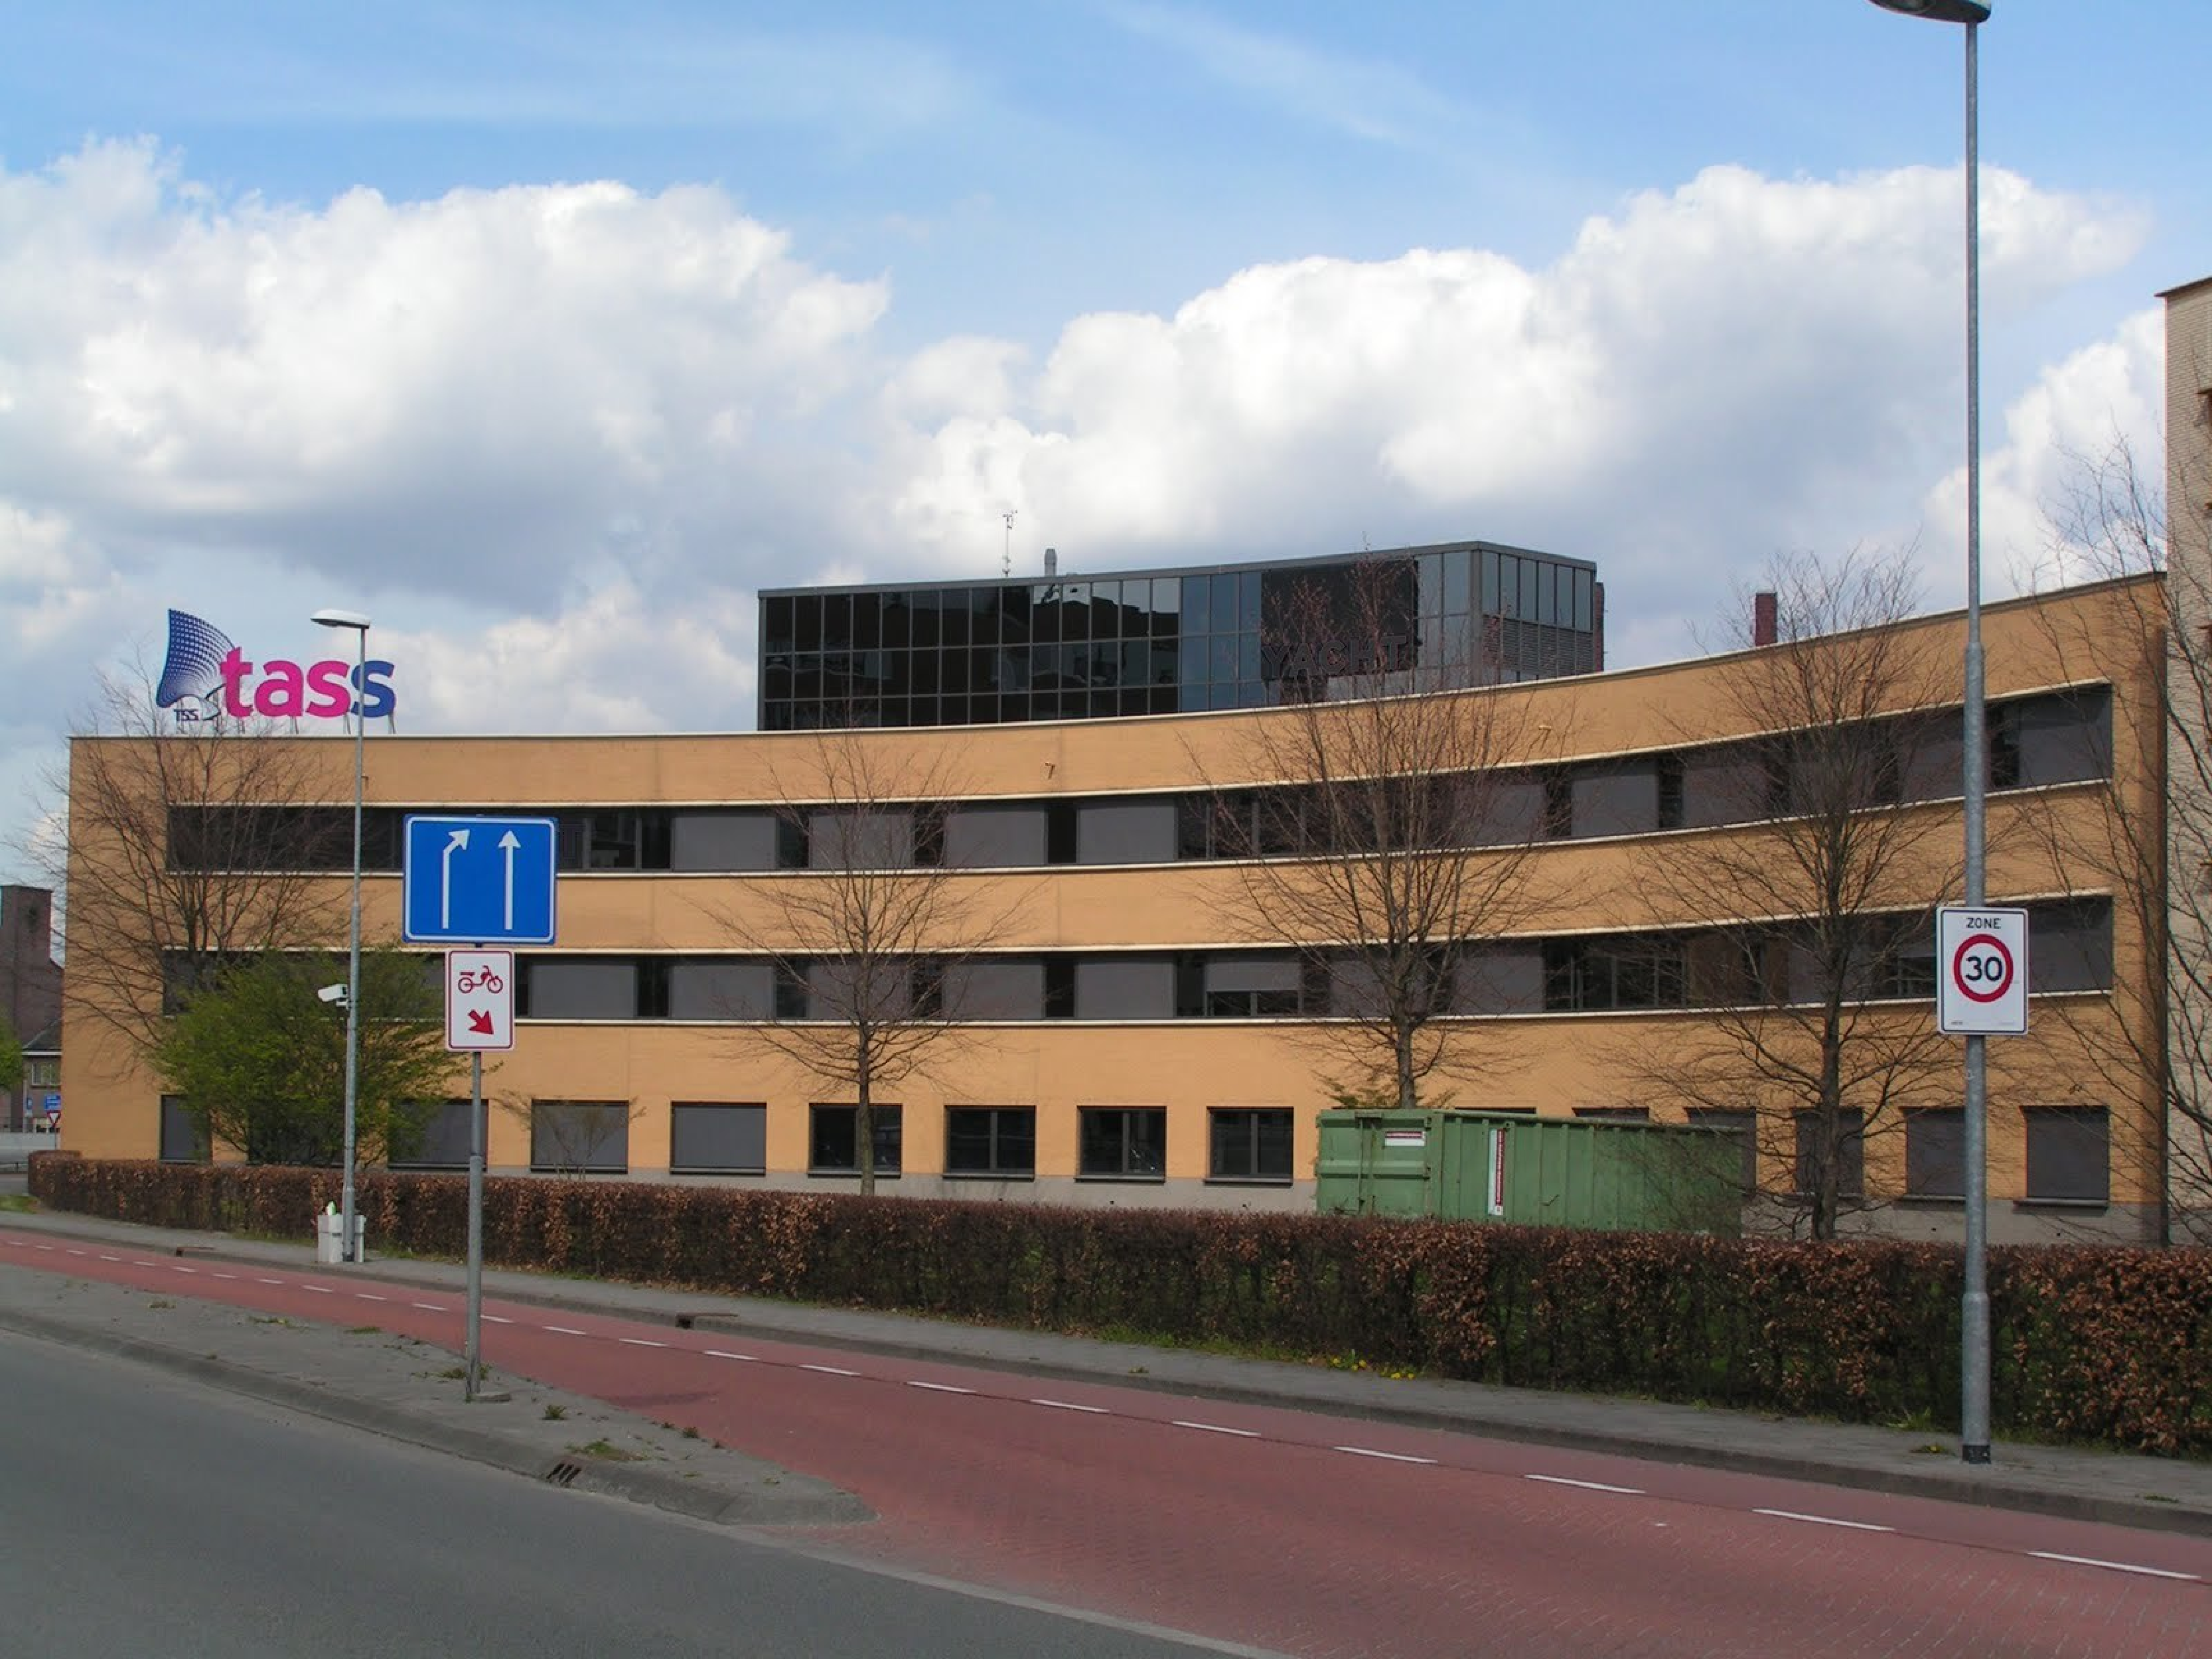
\includegraphics[width=0.40\textwidth]{tass_eindhoven.pdf}
  \end{center}
  \caption{TASS Eindhoven}
\end{wrapfigure}

TASS is een detacheerder wat inhoudt dat al hun personeel werkzaam is bij
andere bedrijven. Zeker gezien hun geschiedenis heeft TASS nog een goede
relatie met vorige moederbedrijf Philips en werkt ook veel met Philips
samen. Andere bedrijven waar veel mee wordt samengewerkt zijn TomTom, ASML
en Bosch.

Buiten het detacheren heeft TASS ook een aantal projecten intern lopen. Het
grootste en meest bekende project is het uCAN[1] project. Dit project
focust zich op het inzichtelijk maken van sensorgegevens uit auto’s. Het
leest de CAN-Bus uit en zendt de informatie door naar een server in de
cloud.

Binnen TASS is het grootste deel van het personeel gedetacheerd bij een
bedrijf. Deze mensen krijgen allemaal een People Manager (PM) toegewezen.
Deze PM zorgt voor de relatie tussen TASS en de medewerker evenals
eventuele problemen tussen de medewerker en het bedrijf waar deze
gedetacheerd zit.

De plek waar de medewerker gedetacheerd is binnengehaald door de account
managers van TASS. Een account manager heeft een aantal bedrijven in
zijn/haar portfolio zitten met wie ze contact hebben over mogelijke
opdrachten voor medewerkers. Mochten ze een plek vinden, zorgen zij voor
een goede kandidaat in samenwerking met de people managers.

Tijdens het afstuderen is er voor de afstudeerder ook een people manager
die het project zal begeleiden, in dit geval is het Gerben Blom. Deze
people manager zal de afstudeerders begeleiden op projectmatig vlak,
functioneren als Project Owner en eventueel antwoord geven op technische
vragen.

Twee wekelijks zal er een review punt komen waar de people manager
samenkomt met de afstudeerder om de voortgang en problemen te bespreken.
Tevens zal daar besproken en getoond worden wat voor producten er deze week
opgelevererd zijn. Hierna zullen ook de taken van de volgende twee weken
bepaald worden en gekeken of daar haken en ogen aan zitten.

Buiten de People Manager krijgen de afstudeerders ook een technische
begeleider toegewezen. Onze hoofd technische begeleider heet Bas Burgers,
maar ook Berry Borgers is erg geïnteresseerd is het DomoTop project en hij
wilt graag onze tweede technische begeleider zijn. De people manager is
niet meer dagelijks bezig met technische ontwikkeling en kan op dat vlak
eventueel achter lopen. De technische begeleider zal vanuit een
gedetacheerde medewerker zijn die nog wel dagelijks bezig is met techniek.
Deze technische begeleider zal zich dan ook niet bezig houden met de
project management zaken maar vooral met de technische problemen of bragen
waar we tegenaan lopen.

\begin{wrapfigure}{l}{0.5\textwidth}
  \begin{center}
    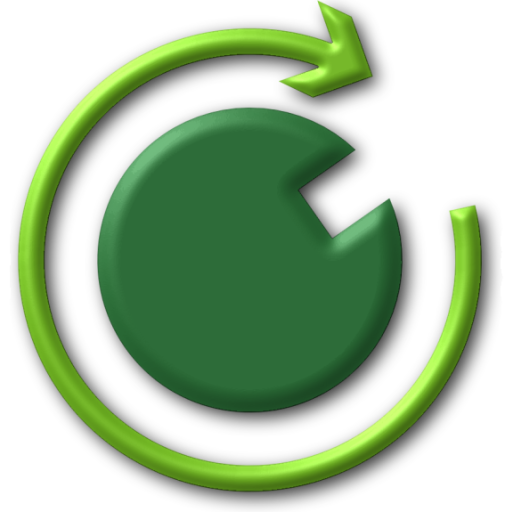
\includegraphics[width=0.20\textwidth]{openremote.pdf}
  \end{center}
  \caption{OpenRemote logo}
\end{wrapfigure}

Het product wat ontwikkeld zal gaan worden is een uitbreiding op een
bestaand open source project, namelijk OpenRemote. OpenRemote zal dan ook
in zekere zin de klant rol vertegenwoordigen. Wij zouden graag zien dat
onze uitbreiding opgenomen zullen worden in OpenRemote en daarvoor moeten
we aan de standaarden voldoen die OpenRemote stelt. We zullen
verantwoording over onze keuzes moeten afleggen aan de mensen van
OpenRemote. Tevens kunnen de mensen van OpenRemote ons helpen en begeleiden
in het proces en dienen als begeleider in het project.

De klant zal in dit project vertegenwoordigd worden door de People Manager
Gerben Blom. Dit zal in dit project niet de enige klant zijn, ook de
ontwikkelaars en gebruikers van het OpenRemote project de rol van klant
fungeren. Dit betekent dat de documentatie van het project hierop aangepast
moet worden, er zal moeten worden gedocumenteerd in het Engels.

Tot slot zijn de afdelingen HR en ICT beheer betrokken met het project. Bij
de HR afdeling worden zaken zoals contracten behandeld. Bij de ICT afdeling
binnen de organisatie moet er gedacht worden aan het bestellen van
hardware, computers opzetten en bij computer gerelateerde problemen of
vragen kan men bij deze afdeling terecht.

\newpage
\section{Probleemanalyse}

\subsection{Probleemsituatie}

Het open source domotica platform OpenRemote is een software pakket wat
gebruikers in staat stelt een domotica systeem op te zetten in huis wat
overweg kan met meerdere domotica protocollen. Dit systeem bestaat uit drie
delen, ten eerste de OpenRemote controller. Deze controller is een stuk
software wat draait op een computer binnen het huis wat door middel van
domotica geautomatiseerd gaat worden.

De controller communiceert rechtstreeks met het tweede onderdeel van het
OpenRemote pakket, namelijk de client applicatie. Er is een Android, iOS en
webapplicatie te downloaden die kan werken met de OpenRemote controller.

De gebruikersinterface van deze applicaties wordt, samen met de logica
erachter, ontworpen via het derde onderdeel: de composer. Deze composer is
een web applicatie die de mogelijkheid geeft tot het ontwerpen van de
client applicatie evenals de het configureren van de actie of acties die
gebeuren als er bijvoorbeeld een knop wordt ingedrukt.

Dit software pakket heeft echter een groot gebrek, het is niet beveiligd
afgezien van een globale gebruikersnaam en wachtwoord voor het hele
systeem. Dit is niet gewenst en onze opdracht is om dit te verhelpen door
er een authenticatie en autorisatie mechanisme aan toe te voegen.

\subsection{Probleemstelling}

Het probleem wat opgelost moet worden is dat onbevoegden makkelijk toegang
kunnen krijgen op een OpenRemote systeem. Voor dit probleem hebben we de
volgende doelstelling geformuleerd: Het implementeren van beveiliging in
OpenRemote, zodat onbevoegden geen toegang kunnen krijgen op het systeem.

Het eerste deelprobleem die te definiëren is over deze probleemstelling is:
Welke beveiligingstechnieken zijn het best te gebruiken in deze situatie?
Deze doelstelling zal onderzocht moeten worden en uiteindelijk moet het
onderzoek geïmplementeerd worden in OpenRemote.

De volgende probleemstelling die opgelost moet worden binnen het project
is: Geselecteerde gebruikers moet toestemming tot het systeem kunnen worden
verleend. Deze probleemstelling gaat meer richting de autorisatie en over
hoe men gebruikers toestemming kan geven tot een systeem.

Het laatste deelprobleem wat opgelost moet worden is: De ontwikkelaars
moeten de code van OpenRemote doorgronden om deze uiteindelijk uit te
kunnen breiden. Voordat er aan de slag kan worden gaan met uitbreiding van
OpenRemote moet de code eerst onderzocht worden.

Voor dit project zal SCRUM gebruikt als ontwikkelmethodiek, omdat het
daarmee makkelijk is een lopend project mee door te ontwikkelen. Voor meer
informatie zie het hoofdstuk “Methoden en Technieken”.

\newpage
\section{Plan van Aanpak}

In dit hoofdstuk wordt er een samenvatting gegeven van het plan  van  aanpak
document, zie het volledige plan van aanpak bijlage  x.  Het  doel  van  het
project is  van  het  om  OpenRemote  te  beveiligen  en  dit  eventueel  te
demonstreren.  De  opdracht  binnen  het  project  is   om   OpenRemote   te
beveiligen. Op dit moment is er geen enkele manier van beveiliging  aanwezig
in OpenRemote. Ook zal er gebruik gemaakt worden van een PlugTop, waarop  de
OpenRemote server komt te draaien. Er zal gebruik gemaakt worden van  SCRUM,
een ontwikkelmethode, wat flexibel is en resulteert in een product dat  veel
meer aan de verwachtingen van de klant voldoet. Meer informatie  over  SCRUM
kan gevonden worden in het hoofdstuk 'Methoden en technieken'.
Er wordt git gebruikt als versiebeheer software en  dat  in  combinatie  met
GitHub, waar de git hosting online geregeld is.  Er  zal  Google  Documenten
gebruikt worden, waarin de documenten geschreven, opgeslagen worden.
Al deze technieken komen ook verder aan bod in het  hoofdstuk  'Methoden  en
technieken'.

In de eerste weken wordt  er  onderzoek  gedaan  over  welke  technieken  er
gebruikt gaan worden, welk platform,  PlugTop  en  protocollen  er  gebruikt
gaan worden. Daarna wordt de PlugTop opgezet samen met een  mobiel  apparaat
(Android)  waarop  OpenRemote  draait.  Er  wordt  een  'Research  Security'
document opgezet, hierin komt een conclusie te staan wat de aanpak wordt  om
OpenRemote het beste  te  beveiligen.  Met  deze  informatie  wordt  er  een
prototype ontwikkeld. Nadat er een volledig werkend  prototype  is,  kan  er
gekeken worden of en waar dit product uitgebreid en verbeterd kan worden.

Zie bijlage x voor de  lijst  van  risico's,  afspraken,  deadlines  en  een
weekplanning.

\newpage
\section{Methoden en Technieken}

Binnen het project zullen er een aantal methoden, technieken en tools
gebruikt worden om het project tot een goed eind te brengen. Hier zullen de
verschillende keuzes voor methoden, technieken en tools toegelicht worden.

\subsection{Ontwikkelmethodiek}
De eerste keuze was voor een ontwikkelmethodiek. De ontwikkelmethodiek
moest een duidelijke voortgang kunnen laten zien door het project heen. De
begeleider vanuit school moet goed op de hoogte gehouden kunnen worden van
de voortgang evenals de bedrijfsbegeleider. SCRUM is, met de review
momenten, hier een mooie techniek voor. Tevens is binnen het bedrijf veel
kennis en expertise over SCRUM.

TASS heeft een interne website[2] opgezet, die Sensei genoemd wordt, waarin
een grote bron aan informatie over SCRUM is opgenomen. Tevens zijn er een
aantal personen binnen het bedrijf SCRUM-experts wat betekent dat vragen of
problemen altijd beantwoord kunnen worden door een van de experts.

Voor de verschillende SCRUM backlogs is ervoor gekozen een spreadsheet te
gebruiken. Er is gekeken naar verschillende software oplossing maar geen
voldeet aan onze verwachtiging. Een eigen spreadsheet heeft veel
flexibiliteit, alles wat er nodig zou zijn kan zelf ingebouwd worden.

Tevens zijn er meerdere burndown charts om de voortgang snel in te kunnen
zien en bij te kunnen houden. Deze burndown charts houden verschillende
elementen van de backlogs bij om op deze manier alles inzichtelijk te
houden.

\subsection{Versiebeheer}
De techniek de we gebruiken om code en document versies bij te houden is
git. Git is een “version control system” net als bijvoorbeeld subversion en
mercurial. Het doel van git is om verschillende versies van bestanden bij
te houden en te kunnen springen in versies. Git heeft als grote voordeel
dat het gedistribueerd is, wat betekent dat elke git clone (vergelijkbaar
met een svn checkout) een volledige geschiedenis met zich mee heeft. Het is
dus niet noodzakelijk een centrale server te gebruiken, al wordt dit vaak
wel gedaan. Dat betekent ook dat elke git clone een backup is van de gehele
geschiedenis.

Om toch een centrale plaats te hebben waar alle verandering naartoe
gestuurd te worden hebben wij ervoor gekozen om Github te gebruiken. Github
is een online platform voor git-repositories, met een erg goede
webinterface. In deze webinterface kan de code ingezien worden, issues
worden aangemaakt en er is een wiki aanwezig.

\subsection{Documenten}
Voor het maken van documenten is er voor gekozen om Google Documenten te
gebruiken. Google Documenten is een web applicatie waarmee eenvoudig en
snel documenten kunnen worden gemaakt. Tevens is het mogelijk om met
meerdere mensen in een document te werken zonder conflicten te krijgen. Ook
de SCRUM spreadsheets staan Google Documenten.

Voor het afstudeerverslag hebben we voor \LaTeX gekozen. Dit omdat het
makkelijker is om de opmaak en uiterlijk te wijzigen en dit meer mogelijkheden
biedt dan het meer beperkt Google Documenten. Ook bestond de wens bij studenten
om meer ervaring op te doen met \LaTeX en dit leek hen de de uitgelezen kans om
dit te doen

\subsection{Programmeertalen}
De talen die gebruikt gaan worden liggen al vast aangezien we verder gaan
werken op een bestaand project. Voor de controller wordt gebruik gemaak van
Java, evenals voor de composer. De verschillende applicaties maken gebruik
van Java op Android en Objective-C op iOS.

\subsection{Database}
Er is gebruik gemaakt van RazorSQL[3], met dit programma is het mogelijk om
SQL queries te maken, typen en de testen via een grafische interface en dit
alles werkt ook met de database die gebruikt wordt bij het DomoTop project,
genaamd HSQLDB[4]. In deze database worden gegevens opgeslagen van de
apparaten die zich aanmelden bij OpenRemote evenals de groepen komen in de
database te staan.  RazorSQL is enkel een tool die gebruikt is bij het
testen/opzetten van de database, daarom is deze tool niet meer
noodzakelijk.

Er is gekozen voor HSQLDB vanwege het feit dat deze database 100% in Java
is geschreven (net als de Controller van OpenRemote), volledig open-source,
HSQLDB heeft een relatief weinig impact op het systeem en is multithreaded.
HSQLDB is namelijk klein en gebruikt weinig bronnen. Tot slot voldoet
HSQLDB aan alle eisen en beschikt over alle mogelijkheden die noodzakelijk
zijn binnen het DomoTop project, denk hierbij aan tabellen aanmaken, rijen
toevoegen, updaten, verwijderen en veel meer. Alternatieven van HSQLDB zijn
niet in native Java code geschreven,  vraagt ook meer van het systeem qua
bronnen en zijn groter als HSQLDB. Sommige alternatieven zijn zelfs niet
eens geschikt om te gebruiken in combinatie met een TomCat server.

\subsection{Ontwikkelomgeving}
Voor de Android applicatie wordt gebruik gemaakt van de Eclipse
ontwikkelomgeving met de ADT plugin. Hiermee is het makkelijk om wijziging
live te draaien op een tablet of een emulator.

Bij het programmeren van de OpenRemote Controller wordt er gebruik gemaakt
van de Eclipse omgeving. OpenRemote Controller is in Java geschreven code
en deze Controller is ook vanaf het begin af aan gestart in de Eclipse
ontwikkeling omgeving. Omdat OpenRemote Controller al ontwikkeld is in
Eclipse, wordt er ook gebruik gemaakt van Eclipse. In Eclipse wordt Ant
Build gebruikt om de Controller te bouwen en compileren. Uiteindelijk krijg
je één WAR bestand, deze WAR kan eenvoudig geïmporteerd worden in de TomCat
Web Application Manager waarna de Controller gebruikt kan worden. TomCat is
de webserver die OpenRemote al gebruikt om de OpenRemote Controller op te
kunnen zetten. Het DomoTop project heeft daarom ook TomCat gebruikt, omdat
dit het meest toegankelijke oplossing is, gezien het feit OpenRemote hier
ook al mee werkt.

Tevens wordt er gebruik gemaakt van een Eclipse plugin genaamd Colorer[5].
Met deze plugin is het mogelijk om syntax highlighting aan te zetten voor
XML (HTML) documenten, maar ook CSS en JavaScript bestanden. Er is hiervoor
gekozen, omdat Eclipse standaard geen highlighting heeft voor bovengenoemde
type bestanden. Desalniettemin is het optioneel om de Eclipse Colorer
plugin te gebruiken, het is enkel gekozen voor gemaks doeleinden.

\subsection{Libraries}
Om in Java met encryptie en TLS te kunnen werken in native Java code wordt
er gebruik gemaakt van Bouncy Castle wat een gratis open-source software.
Bouncy Castle is een bibliotheek die binnen het project onder andere
gebruikt wordt om nieuwe certificaten te kunnen generen vanuit Java code
alsmede een CSR bestand uit te lezen en deze gegevens gebruiken om een
nieuw certificaat te onderteken door middel van een CA. Ook het gebruikte
CA certificaat wordt aangemaakt door middel van Bouncy Castle. Ook onder 
Android wordt er gebruik gemaakt van de Bouncy Castle bibliotheek, echter 
heet dat onder Android Spongy Castle, maar is exact dezelfde code.

In de OpenRemote Controller is er gebruikt gemaakt van een template engine
genaamd Freemarker[6]. Deze template engine maakt het mogelijk om statische
opmaak (template design) te scheiden van dynamisch gegevens zoals apparaat
gegevens uit een database. Freemarker werkt goed samen met Java en TomCat.
Verder is FreeMaker een relatief kleine template engine en simpel te
begrijpen maar toch doeltreffend. FreeMarker forceert zich op het gebruik
van een Model View Controller software architectuur. FreeMarker wordt ook
vaak gebruikt voor servlet gebaseerde web applicatie ontwikkeling en dat is
exact wat de OpenRemote Controller is.

\newpage
\section{Uitvoering}

\begin{wrapfigure}{r}{0.5\textwidth}
  \begin{center}
    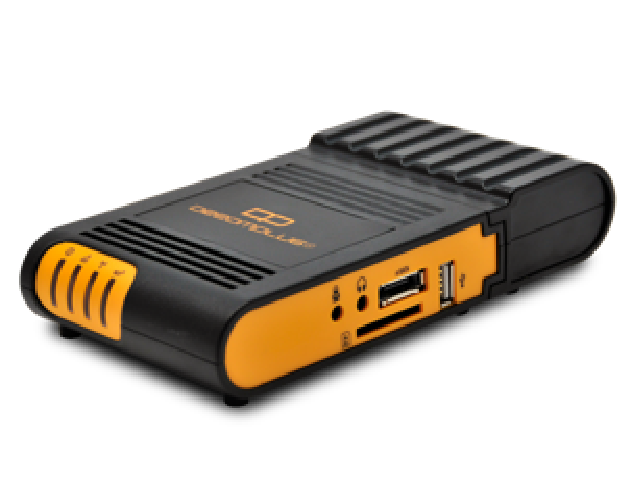
\includegraphics[width=0.50\textwidth]{dreamplug.pdf}
  \end{center}
  \caption{Een PlugTop computer}
\end{wrapfigure}

Het begin van de stage stond in het teken van onderzoek. Er was bij ons
weinig kennis van het domotica veld, OpenRemote, PlugTop computers en
beveiliging dus al deze velden moesten onderzocht worden. Het project begon
met een globaal onderzoek naar het domotica veld en PlugTop computers. Alle
onderzoeken zijn gedocumenteerd in verschillende documenten die te vinden
zijn in de bijlages. Het volgende onderzoek wat is gehouden was naar het
OpenRemote software pakket en eventuele alternatieven.

Het laatste onderzoek wat is gedaan is naar de beveiligingstechnieken die
bestaan. Voordat het onderzoek begon, is er een gesprek gehouden met Berry
Borgers aangezien hij al veel kennis had over het beveilingsgebied. De
keuzes die zijn gemaakt in het document is in overleg met Berry Borgers
gebeurd. Dit onderzoek is gedocumenteerd in het Engels zodat het
makkelijkst te delen is met de ontwikkelaars van OpenRemote.

Na het onderzoek is er begonnen met het ontwikkelen van de gekozen
oplossing: TLS te implementeren in OpenRemote om OpenRemote veiliger te
maken. Dit gebeurd door een apparaat een aanvraag laat doen bij de
OpenRemote Controller, de OpenRemote Controller kan deze aanvraag
goedkeuren en het apparaat ontvangt vervolgens het client certificaat. Dit
client certificaat wordt vervolgens gebruikt in combinatie met een apparaat (zoals
Android), waarna er toestemming wordt verleend om de OpenRemote Controller te gebruiken.

Het is noodzakelijk om zowel de OpenRemote Controller alsmede de OpenRemote applicatie 
van Android te modificeren. De aanpak was om allereerst alles op de server, waar ook de 
OpenRemote Controller draait, te maken en genereren. Het CSR bestand wordt
aangemaakt \& ondertekend op de server en ook het
client certificaat wordt gegenereerd op de server. Omdat het belangrijk is
dat alles werkt, wordt er gebruik gemaakt van het openssl commando in de
terminal onder Linux. De certificaten die gegenereerd worden, worden
toegevoegd aan de truststore die TomCat gebruikt. Toen alles eenmaal
werkte bleek al snel dat TomCat telkens moest worden herstart om de
truststore opnieuw uit te kunnen lezen.\\
Om dat probleem op te lossen, zodat TomCat server niet telkens opnieuw
herstart hoefde te worden, is er gekozen om een eigen 'self-signed' CA te
gebruiken. Hiervoor moet enkel het CA certificaat toegevoegd worden aan de
truststore van TomCat en zolang de client certificaten ondertekend worden
door hetzelfde CA certificaat is het mogelijk om de oorsprong van het
client certificaat te achterhalen. Indien het client certificaat inderdaad
getekend is ook de CA, die aanwezig is in de truststore van TomCat, vertrouwd
TomCat deze client en krijgt het apparaat toegang tot de OpenRemote
Controller.

\begin{wrapfigure}{l}{0.5\textwidth}
  \begin{center}
    
\includegraphics[width=0.30\textwidth]{tomcat.pdf}
  \end{center}
  \caption{Het TomCat logo}
\end{wrapfigure}

Omwille van het bovenstaande idee tot een goed einde te brengen is het noodzakelijk dat er onder Android
onderzochtwordt hoe er een client CSR file gemaakt kan worden en hoe het client
certificaat vervolgens geïmporteerd kan worden in de keystore van Android. Op de
server waar ook de OpenRemote Controller draait werd er gekeken hoe je een
CA aanmaakt voor de TomCat server, hoe je client certification request
files kan omzetten in normale client certificaten die ondertekend zijn door
het CA certificaat. En hoe je de client certificaten vervolgens kan opslaan
in één keystore op de server, zodat er op een later termijn nog steeds
informatie opgevraagd kan worden over een client certificaat. Op de server
en de OpenRemote controller werkte dit eerst via het openssl
commando, later is deze code in zijn geheel omgeschreven in native Java
code en wordt er gebruik gemaakt van de Bouncy Castle bibliotheek.

Uiteindelijk is er een grafische interface gemaakt om apparaten goed en/of
af te keuren vanuit de 'administrator panel'. Er bestaat een pin die
vergeleken kan worden met de pin die aanwezig is op het Android apparaat,
indien de pins van Android en de administrator panel overeenkomen, is er
met zekerheid te zeggen dat het hetzelfde apparaat betreft. Naast 'User
management' heeft de administrator panel ook een tab genaamd
'Configuration'. In deze tab is het mogelijk om bepaalde instellingen te
veranderen zoals of de authenticiteit of pin check aan- of uitgezetten. 
De administrator panel is beveiligd door een gebruikersnaam en wachtwoord 
die overeen moet komen met een bestaand OpenRemote Designer account.
Op deze manier is het administratie paneel enkel toegankelijk voor de administrator.

\begin{figure}[htpb]
   \begin{center}
     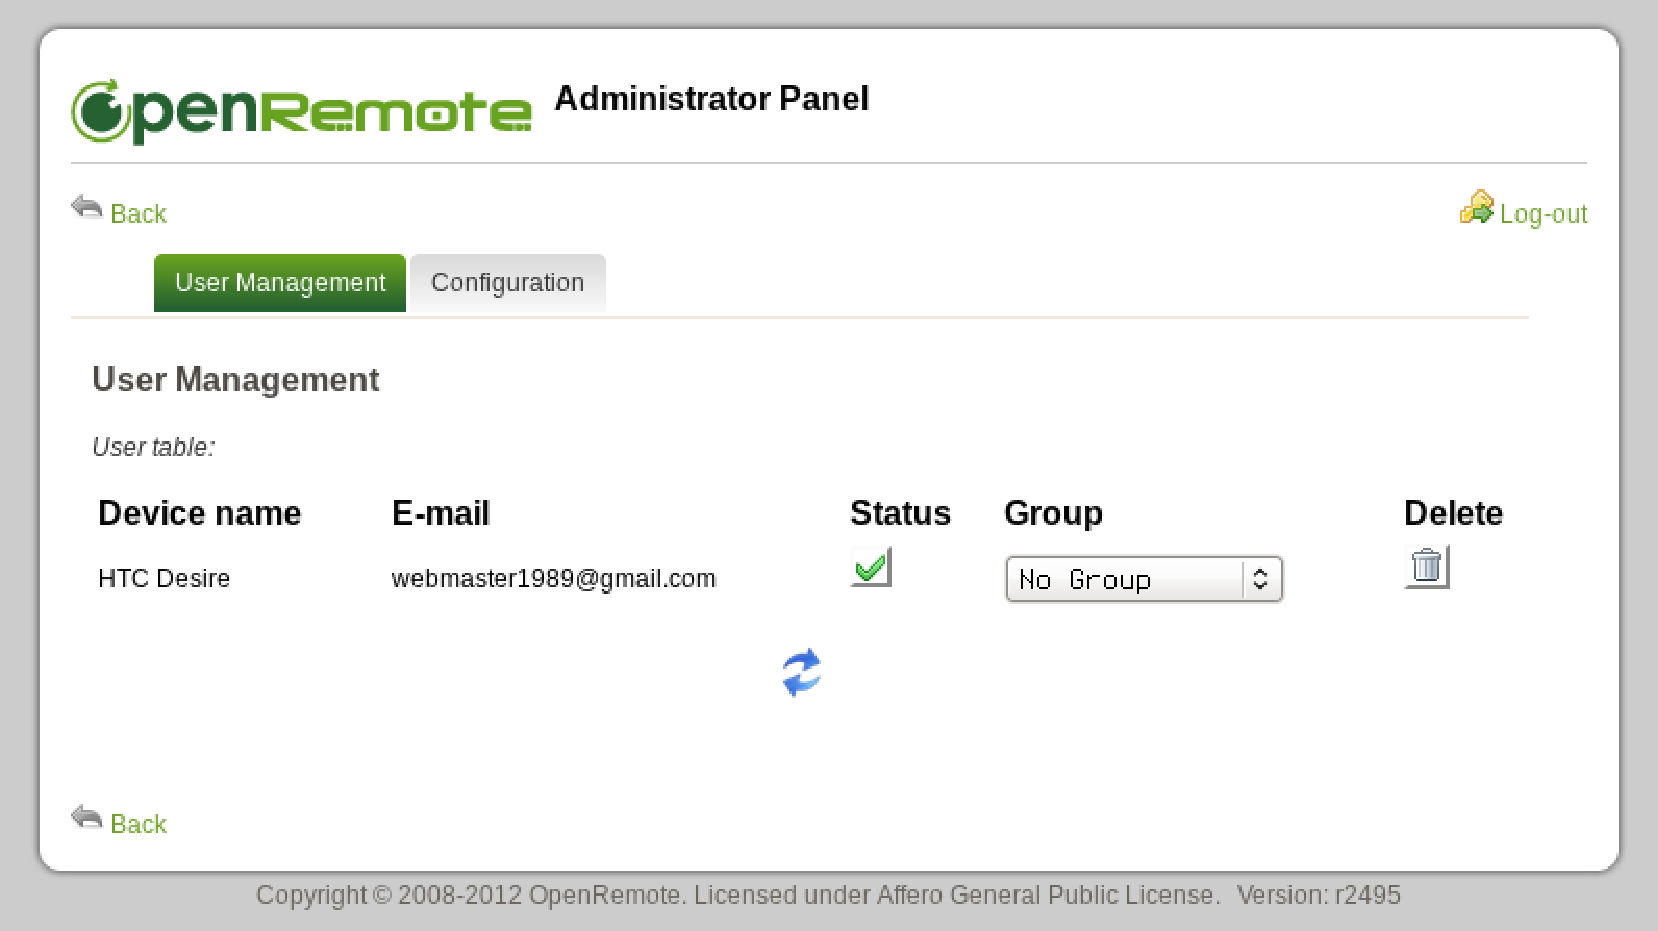
\includegraphics[width=0.6\textwidth]{userlist.pdf}
   \end{center}
   \caption{Gebruikers management lijst}
\end{figure}

\newpage
\section{Resultaten}

Zoals al eerder vermeld, wordt er in het project gewerkt met de SCRUM
ontwikkeltechniek. Deze ontwikkeltechniek werkt met verschillende iteraties
waar verschillende requirements afgerond worden. Na afloop van een iteratie
kunnen er veranderingen aangebracht worden in de lijst met eisen. Hier zal
per iteratie besproken worden wat de eisen waren van van de desbetreffende
iteratie en welke resultaten deze heeft opgeleverd.

\subsection{Iteratie 1}
De eerste iteratie was het vooral belangrijk om onderzoek te doen in het
werkveld waar in gewerkt zou gaan worden de komende weken. Er waren vier
delen waar onderzoek naar gedaan is namelijk: Domotica protocollen,
domotica hardware, plugtops en OpenRemote.

\begin{table}[htpb]
  \caption{Eisen iteratie 1}
  \begin{center}
    \begin{tabular}{|| l ||}\hline
        Eis                                                  \\\hline\hline
        Uitzoeken protocollen en onderzoeksdocument opzetten \\\hline
        Uitzoeken PlugTop en onderzoeksdocument opzetten     \\\hline
        Uitzoeken Hardware en onderzoeksdocument opzetten    \\\hline
        Uitzoeken OpenRemote en onderzoeksdocument opzetten  \\\hline
    \end{tabular}
  \end{center}
\end{table}

Na deze sprint zijn er een aantal documenten opgesteld die duidelijk maken
welke keuzes gemaakt kunnen worden. De conclusie van het protocollen en
hardware onderzoek was dat X10 een mooi en makkelijk te gebruiken protocol
is. Z-Wave is een erg mooi draadloos protocol maar dit wordt minder goed
ondersteund en is duurder waardoor het minder geschikt was voor dit
project.

Het PlugTop onderzoek heeft aangetoond dat de al binnen TASS gebruikte
DreamPlug de meest geschikte PlugTop is voor dit project. De DreamPlug
beschikt over veel aansluiting en is gunstig geprijsd.

In het onderzoek naar OpenRemote is gekeken naar de mogelijkheden van het
OpenRemote in vergelijking met andere software pakketten. Hier is uit
gebleken dat OpenRemote beschikt over de meeste mogelijkheden en het meest
actief wordt bijgehouden. Wel is de beveiliging van OpenRemote niet heel
goed geregeld.

\subsection{Iteratie 2}
\begin{table}[htpb]
  \caption{Eisen iteratie 2}
  \begin{center}
    \begin{tabular}{|| l ||}\hline
        Eis                                                              \\\hline\hline
        Als gebruiker wil ik een Android applicatie om een lamp aan en   \\ 
        uit zetten                                                       \\\hline
        Als klant wil ik weten wat voor authorisatie en authenticatie    \\
        methoden er bestaan.                                             \\\hline
    \end{tabular}
  \end{center}
\end{table}

Tijdens de tweede iteratie is er gewerkt aan het opzetten van een
testopstelling met OpenRemote, de DreamPlug en de X10 hardware. Ook is er
onderzoek gedaan naar verschillende beveilingsmethodieken en oplossingen.

Met de test opstelling kon aan het eind van de iteratie een lamp
aangestuurd worden met de OpenRemote controller, welke moest draaien op de
DreamPlug, met de OpenRemote app om een lamp aan te zetten via een X10
stopcontactmodule.

Het onderzoek over beveiliging concludeert dat de beste methode om
OpenRemote te beveiligen het gebruiken van SSL certificaten is. Deze
certificaten kunnen door zowel de server als de client gebruikt worden om
zich te authenticeren.

\subsection{Iteratie 3}
De derde iteratie stond in het teken van de Proof-of-Concept die laat zien
dat het mogelijk is om met Android te verbinden naar een TomCat server en
te authenticeren door middel van SSL Client Certificaten.

\begin{table}[htpb]
  \caption{Eisen iteratie 3}
  \begin{center}
    \begin{tabular}{|| l ||}\hline
        Eis                                                              \\\hline\hline
        Als beheerder wil ik zien welke apparaten er zijn aangemeld      \\\hline
        Als systeem wil ik onderscheid zien tussen verschillende devices \\\hline
        Als gebruiker wil ik zien dat mijn telefoon uniek                \\ 
        identificeerbaar is                                              \\\hline
    \end{tabular}                                                         
  \end{center}                                                            
\end{table}                                                               

Voor de Proof-of-Concept waren een aantal eisen. Als eerste moet de client
een aanvraag kunnen doen bij de server voor een certificaat. Deze aanvraag
moet in een lijstje te zien zijn waarna er een certificaat terug wordt
gestuurd naar de client. Dit certificaat wordt gegenereerd op de server en
Base64 geencodeerd en overgestuurd naar de client.

De beheerder kan op de server een lijst met aanvragen zien evenals een
lijst met gebruikers die daadwerkelijk een certificaat hebben. Na deze
sprint was het nog niet mogelijk om dynamisch gebruikers een certificaat te
geven en werd dit automatisch gedaan. De lijst met clients die een aanvraag
hebben gedaan zal dus dezelfde zijn als de clients met een certificaat.

De telefoon van de gebruiker moest uniek identificeerbaar zijn. De server
en client moest kunnen zien dat de client uniek identificeerbaar is. Er
moest dus een manier gevonden worden waar de server aan kon zien welke
client er verbonden is. Hiervoor is het ``serial'' attribuut van het client
certificaat gebruikt. Dit attribuut is een oplopend nummer welke in elk
certificaat aanwezig is.

\subsection{Iteratie 4}
In de daaropvolgende iteratie is er gewerkt aan het implementeren van de
Proof-of-Concept in het OpenRemote project.

Er waren een aantal onderdelen die verbeterd moesten worden wanneer ze
geimplementeerd zouden worden in het OpenRemote project. De beheerders
interface was een onderdeel hiervan. Deze interface is verbeterd, hij is
ontworpen (zie figuur ~\ref{fig:adminv1}) en er zijn acties aangekoppeld waarmee de client
goedgekeurd kan worden.

\begin{table}[htpb]
  \caption{Eisen iteratie 4}
  \begin{center}
    \begin{tabular}{|| l ||}\hline
        Eis                                                              \\\hline\hline
        Als beheerder wil ik sommige gebruikers toestemming geven in een \\ 
        webinterface                                                     \\\hline
        Als gebruiker wil ik met de android app van OpenRemote client    \\ 
        certificaten gebruiken om te verbinden met de server             \\\hline
        Als gebruiker wil ik met de android app van OpenRemote een client\\
        certificaat op kunnen halen van de server                        \\\hline
        Als beheerder wil ik een lijst zien in met gebruikers in een     \\ 
        webpagina op de openremote controller                            \\\hline
        Als beheerder wil ik clients toestemming kunnen geven door middel\\ 
        van een PIN uit te wisselen en te controleren in de web interface\\\hline
    \end{tabular}
  \end{center}
\end{table}

Van deze clients kan informatie getoond worden, namelijk het email adres,
de naam van de telefoon en een PIN. Deze PIN wordt gegenereerd door een
hash van de publieke sleutel te maken en daarvan de laatste 4 karakters te
laten zien.

\begin{figure}[h!]
  \centering
    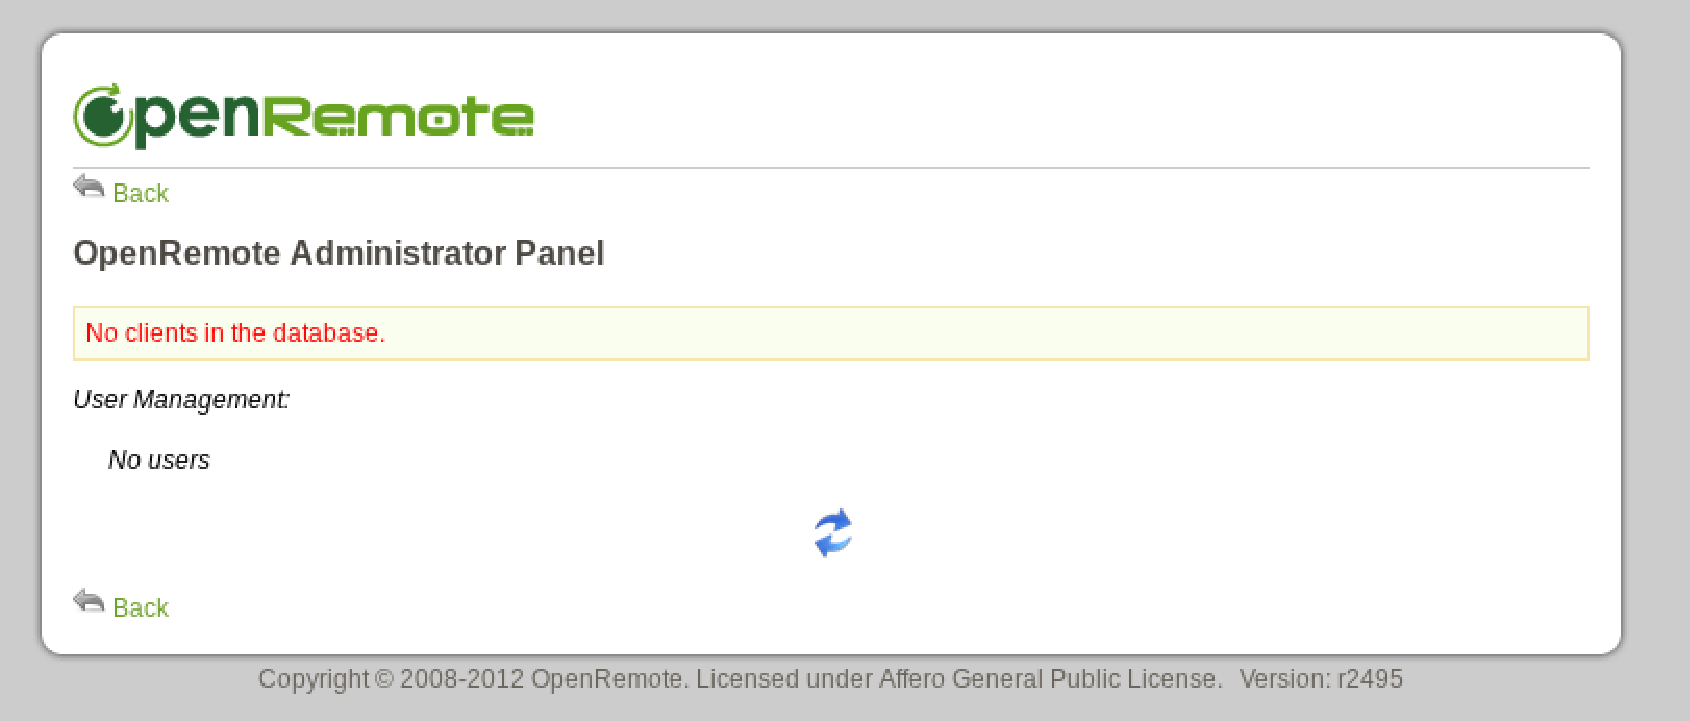
\includegraphics[height=150pt,keepaspectratio]{adminv1.pdf}
  \caption{Ontwerp beheerderspanel}
  \label{fig:adminv1}
\end{figure}

De app stuurt sinds deze iteratie een CSR naar de server die de server
gebruikt om een certificaat te maken. Op deze manier wordt de private
sleutel van de client nooit overgestuurd en kan deze ook niet onderschept
worden door kwaadwillenden.

\subsection{Iteratie 5}
\begin{table}[htpb]
  \caption{Eisen iteratie 5}
  \begin{center}
    \begin{tabular}{|| l ||}\hline
        Eis                                                              \\\hline\hline
        Als beheerder wil ik in kunnen loggen met de gegevens van        \\
        http://composer.openremote.org                                   \\\hline
        Als beheerder wil ik de toegang van clients kunnen intrekken van \\ 
        het systeem om de toegang te ontzeggen                           \\\hline
        Als beheerder wil ik de OpenRemote Controller op alle            \\ 
        verschillende platformen kunnen installeren                      \\\hline
        Als gebruiker wil ik de interface zo simpel mogelijk maken       \\\hline
    \end{tabular}
  \end{center}
\end{table}

De vijfde iteratie kwam het probleem van platform ondersteuning om de hoek.
OpenRemote is een cross platform applicatie. De Controller draait op TomCat
welke in Java geschreven is. Dit betekent dat het draait op elk platform waar
java draait. Echter hebben de wijzigingen die in de vorige iteratie zijn
doorgevoergd er voor gezorgd dat het nu noodzakelijk is toegang te hebben tot
het 'openssl' commando. In deze iteratie is er voor gezorgd dat dit niet meer
nodig is. Voor alle cryptografische acties wordt nu gebruik gemaakt van Bouncy
Castle library. 

In figuur ~\ref{fig:tls} is te zien wat er nu precies gebeurd als er een
aanvraag binnenkomt bij de Controller. De client doet in het begin een aanvraag
voor toegang. Hiermee stuurt hij een CSR bestand op waar al zijn gegevens in staan,
welke de Controller gebruikt om een certificaat te maken. 

Als er een aanvraag binnen komt voegt de Controller de nieuwe client toe aan de
database. De gegevens in de database worden uit de CSR gehaald. Als dit allemaal
gedaan is, is de client te zien in de beheerdersinterface. Hij is nog niet
goedgekeurd en heeft dus ook geen toegang tot het systeem.

Wanneer de beheerder de client goedgekeurd heeft, en desgewenst de pin ingevoerd
heeft, wordt het proces gestart om een certificaat te genereren. Als eerste
wordt de private sleutel van de CA opgehaald. Elk certificaat dat gemaakt wordt,
wordt ondertekend door de CA. Deze CA wordt ook geimporteerd in de OpenRemote
Controller en op die manier weet OpenRemote dat hij de clients kan vertrouwen.

Daarna wordt de private sleutel samen met de CSR gebruikt om een certificaat te
cree"eren. Tevens moet er een serienummer meegegeven. Dit serienummer is een
uniek oplopend nummer waarmee de certificaten makkelijk te identificeren is. Het
certificaat wat dan gemaakt is wordt het certificaat een in een keystore
opgeslagen, klaar om opgehaald te worden door de mobiele applicatie en wordt de
status van de client in de database aangepast.

Nu kan de client met de applicatie een certificaat ophalen en met dit
certificaat een veilige verbinding opzetten. Tevens kan TomCat het certificaat
gebruiken om de gebruiker te identificeren. In de database staat de ``dname''
welke ook in het certificaat staat. Op het moment dat een client een verbinding
maakt met TomCat, controleert TomCat de dname en kijkt in de database of deze
gebruiker toegang heeft tot het systeem. Mocht dat niet het geval zijn, zal hij
de gebruiker geen toegang tot het systeem geven.


\begin{landscape}
\begin{figure}[h!]
  \centering
    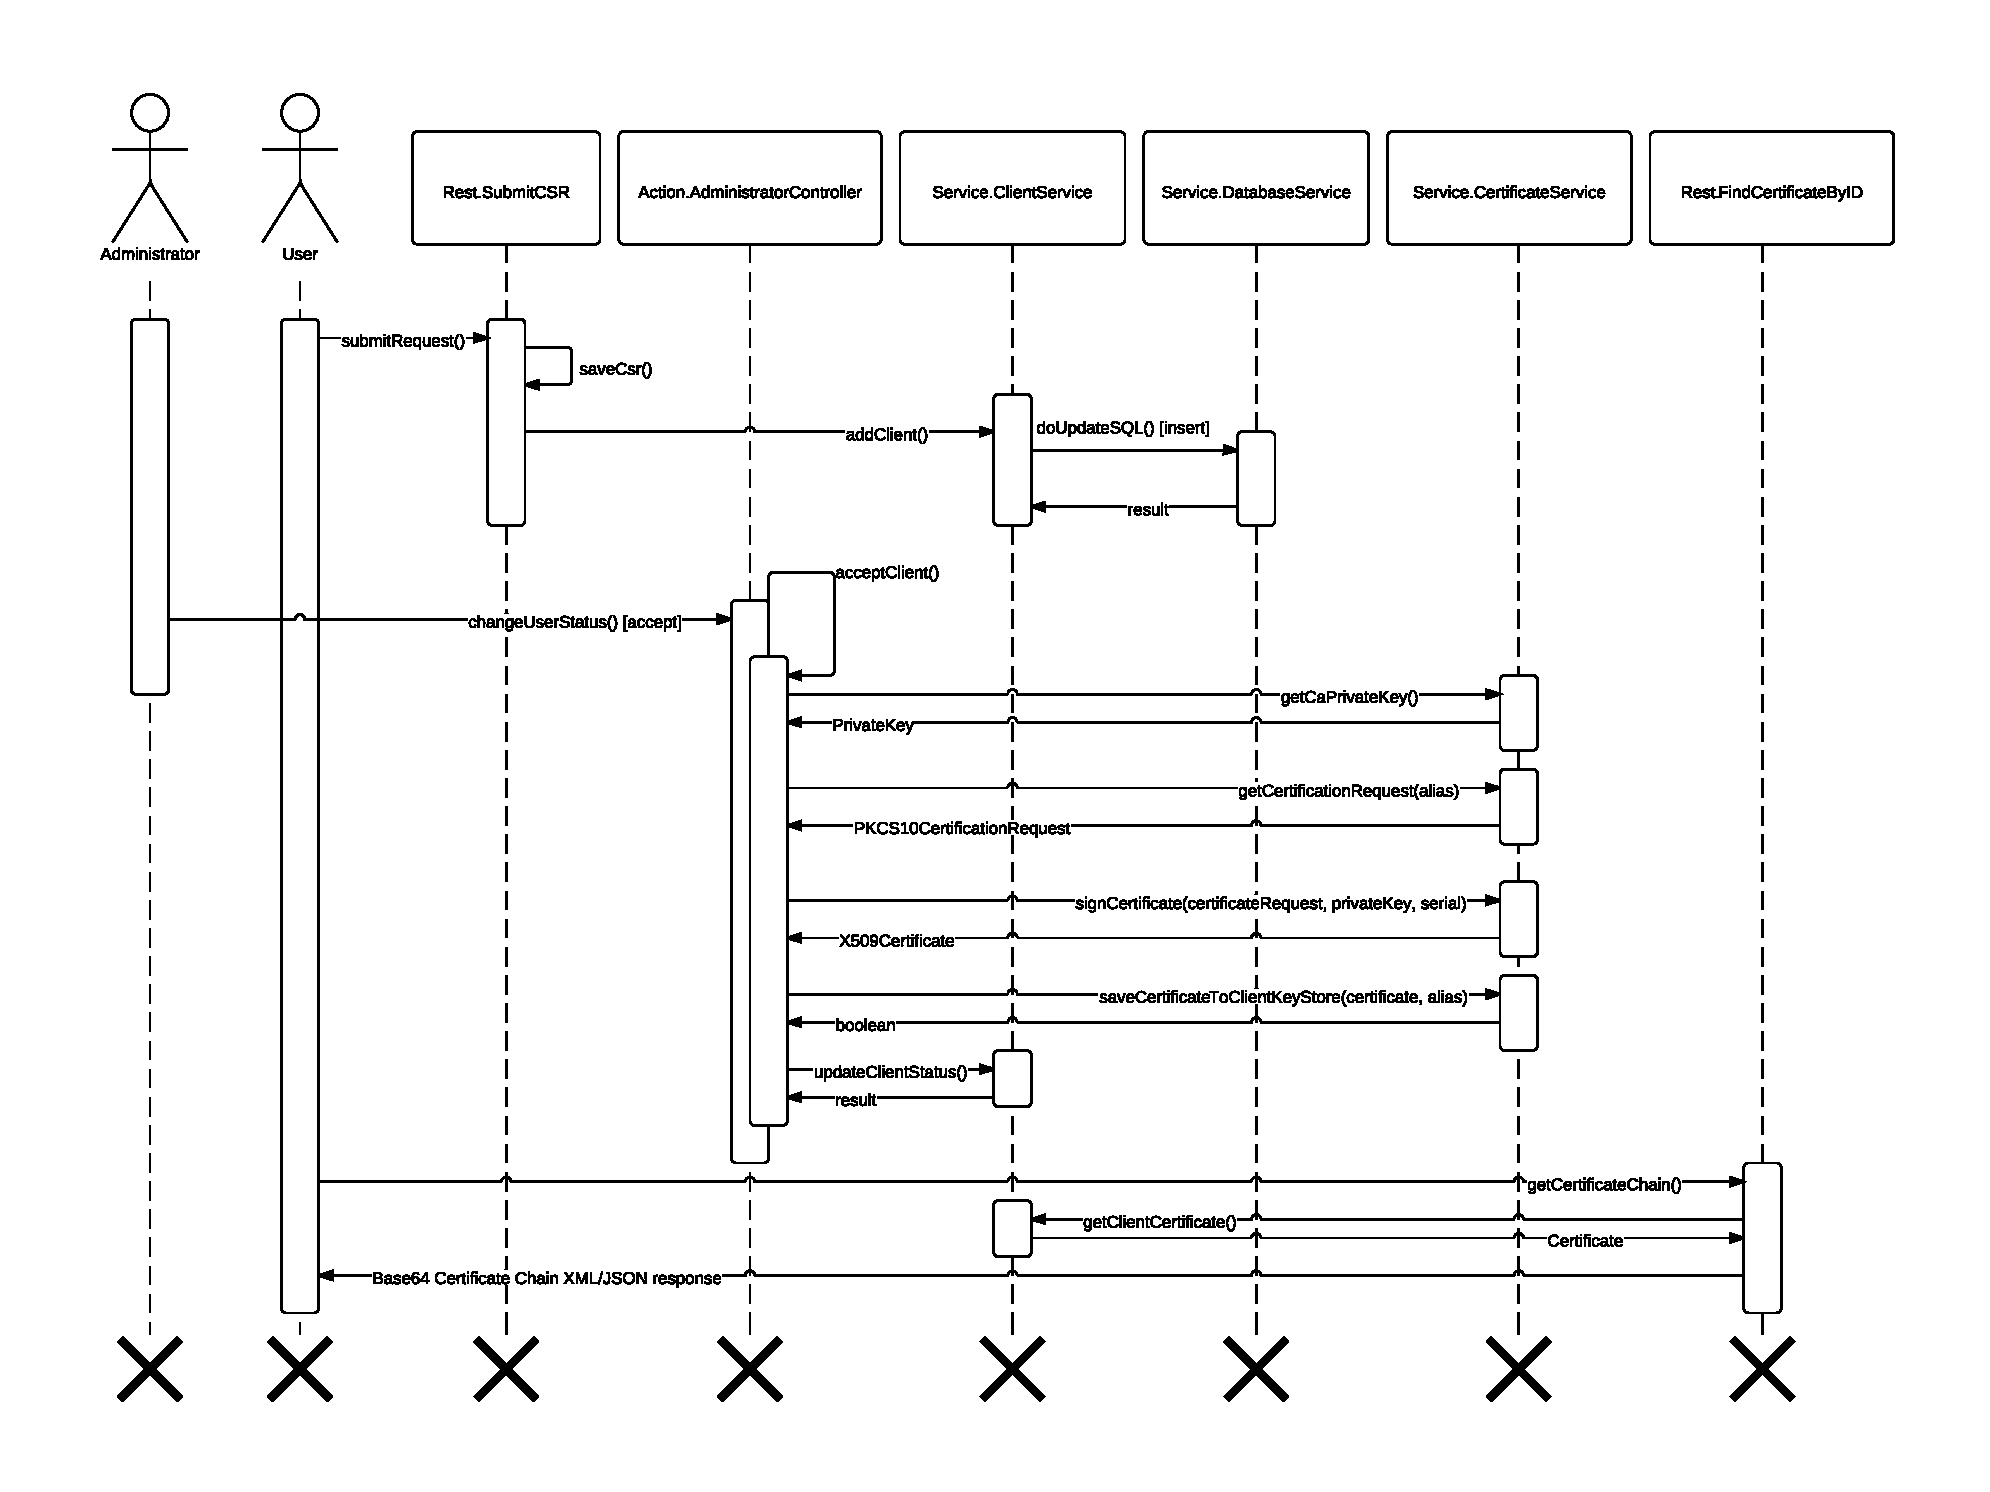
\includegraphics[height=1\textheight,keepaspectratio]{DomoTopSequenceDiagram_without_title.pdf}
  \label{fig:tls}
  \caption{DomoTop Sequence Diagram - Afhandelen van een request via een TLS
  capable OpenRemote Controller}
\end{figure}
\end{landscape}

Om een aantal dingen te kunnen aanpassen als beheerder is er ook een
configuratiescherm gemaakt. In dit scherm kunnen een aantal dingen worden
ingesteld zoals onder andere het pad waar de CA opgeslagen wordt en of de PIN
verplicht gecontroleerd moet worden.

\begin{figure}[h!]
  \centering
    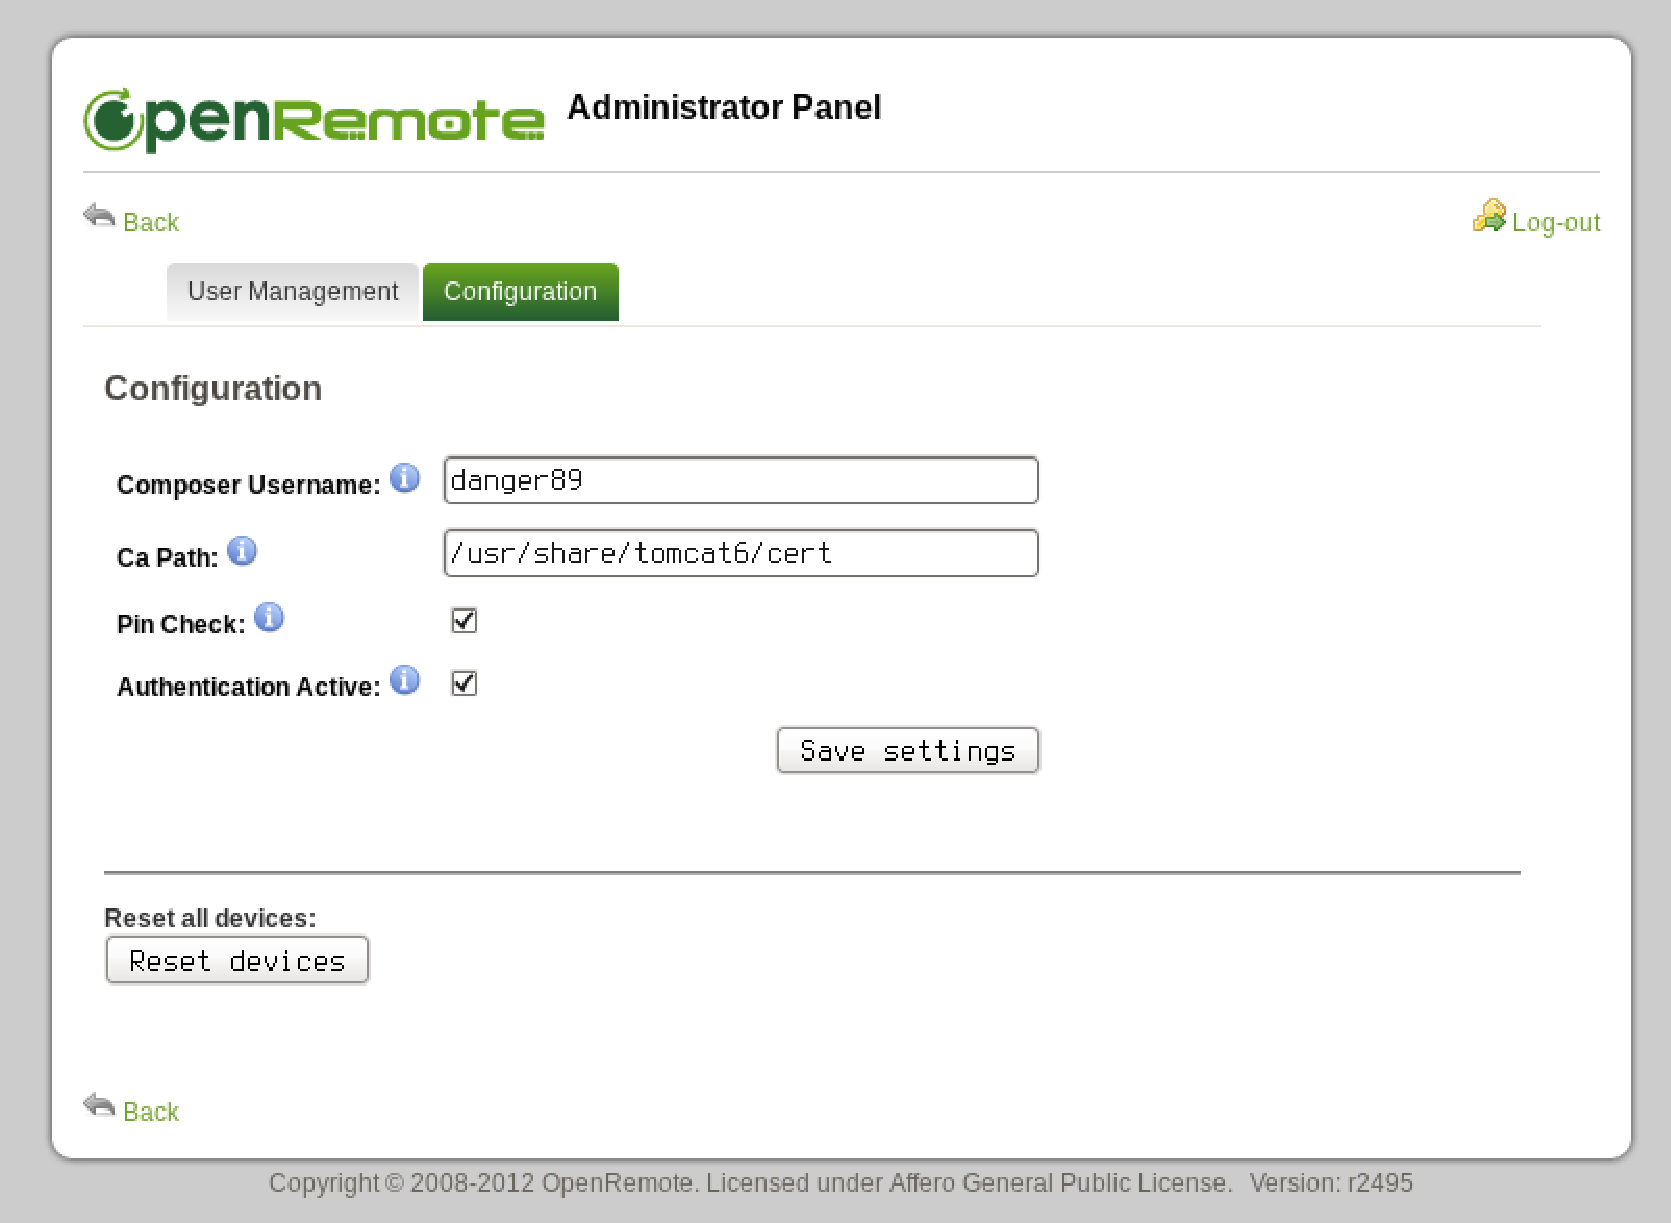
\includegraphics[width=1\textwidth,keepaspectratio]{adminv2config.pdf}
  \label{fig:adminv2config}
  \caption{Het configuratiescherm}
\end{figure}

Dit configuratiescherm en het user management scherm zijn beide beveiligd met
een gebruikersnaam en wachtwoordcombinatie. Deze combinatie is dezelfde als
waarmee ingelogd wordt op \url{http://composer.openremote.org/}. Deze worden,
wanneer er ingelogd wordt gecontrolleerd online of, als er geen
internetverbinding is, lokaal met de cache die te vinden is in de database.

\newpage
\section{Verklarende woordenlijst}

\begin{longtable}{|| l | l ||}\hline
    Begrip           & Omschrijving                                         \\\hline\hline
    CAN-Bus          & CAN-bus is een standaard voor in voertuigen ontworpen\\
                     & om microcontrollers en apparaten met elkaar te       \\
                     & communiceren zonder een host-computer.               \\\hline
    OpenRemote       & Een domotica pakket waarmee je meerdere domotica     \\
                     & protocollen aan kan sturen                           \\\hline
    Android          & Een besturingssysteem voor mobiele telefoons en      \\
                     & tablets gemaakt door Google                          \\\hline
    iOS              & Een besturingssysteem voor mobiele telefoons en      \\
                     & tablets gemaakt door Apple                           \\\hline
    GitHub           & Een online git hosting platform                      \\\hline
    SCRUM            & Een ontwikkelmethodiek die werkt met meerdere        \\
                     & iteraties om zo klantvriendelijk te kunnen           \\
                     & ontwikkelen.                                         \\\hline
    PlugTop          & Een energiezuinige computer in het formaat van een   \\
                     & forse adapter.                                       \\\hline
    Multithreaded    & Meer dan één thread, dit kan de efficient van de     \\
                     & hardware tegoede komen.                              \\\hline
    CA               & CA staat voor Certificate authority en is bedoeld om \\
                     & certificaat aanvragen goed te keuren en een          \\
                     & certificaten te beheren en te generen.               \\\hline
    TomCat Web       & TomCat heeft een Web Application Manager waarbij je  \\
    Application      & eenvoudig via een web interface je applicaties (WAR  \\
    Manager          & bestanden) te beheren, updaten, uploaden.            \\\hline
    Java Servlet     & Een servlet is een in Java geschreven programma dat  \\
                     & op een server draait. De servlet maakt hierbij       \\
                     & gebruik van een aantal diensten die de               \\
                     & webcontainer biedt, zoals het afhandelen van de      \\
                     & communicatie met de client.                          \\\hline
    Model View       & Model-view-controller (of MVC) is een ontwerppatroon \\
    Controller       & dat het ontwerp van complexe toepassingen opdeelt in \\
    software         & drie eenheden met verschillende                      \\
    Architectuur     & verantwoordelijkheden: datamodel, datapresentatie en \\
                     & applicatielogica. Het scheiden van deze              \\
                     & verantwoordelijkheden bevordert de leesbaarheid en   \\
                     & herbruikbaarheid van code.                           \\\hline
    KeyStore         & Een Java keystore (JKS) is een bestand waar          \\
                     & beveiligingscertificaten, aanvraag certificaten of   \\
                     & publieke sleutels worden opgeslagen                  \\
                     & - wat gebruikt wordt met SSL encryptie.              \\\hline
    TrustStore       & Zie: KeyStore, een TrustStore bevat certificaten     \\
                     & die zijn geaccepteerd om verbinding mee op te zetten.\\
                     & Of een CA ceritificaat waarbij de ondertekende       \\
                     & certificaten vertrouwd  zijn.                        \\\hline
    Self-signed      & Een certificaat kan self-signed zijn,                \\
                     & wat erop duidt dat het certificaat door zichtzelf    \\
                     & ondertekend is.                                      \\\hline
    Proof-of-Concept & Een applicatie die laat zien dat een bepaalde        \\
                     & techniek gebruikt kan worden. Deze applicatie laat   \\
                     & alleen zien dat de techniek werkt.                   \\\hline
    CSR              & Certification Sign Request, met behulp van dit       \\
                     & bestand kan de CA een certificaat genereren.         \\\hline
\end{longtable}

\newpage
\section{Bronnen}

\newpage
\section{Bijlagen}

In dit hoofdstuk komen de bijlagen te staan. Elke bijlage is genummerd en
dit nummer kan worden in het document als referentie.

\subsection{Bijlage 1: Plan van Aanpak}

\newpage
\section{Verantwoording individuele bijdrage}

\begin{tabular}{|| l | c | c ||}\hline
    Onderdeel           &   \multicolumn{2}{|c||}{Verantwoordelijke} \\\hline
                        & Melroy van den Berg & Vincent Kriek        \\\hline\hline
    Hoofdstuk 1         &                     &  X                   \\\hline
    Hoofdstuk 2.1       &                     &  X                   \\\hline
    Hoofdstuk 2.2       &                     &  X                   \\\hline
    Hoofdstuk 3         &       X             &                      \\\hline
    Hoofdstuk 4         &       X             &  X                   \\\hline
    Hoofdstuk 5         &       X             &                      \\\hline
    Hoofdstuk 6         &                     &  X                   \\\hline
\end{tabular}


\end{document}
